%!TEX root = syntheyes15.tex

\section{Synthetic data generation}

In this section we first present our anatomically inspired CG eyeball model, and then explain our novel procedure for preparing a suite of 3D head scans for dynamic photorealistic labelled data generation. We then briefly describe how we use image-based lighting \cite{debevec2002image} to model a wide range of realistic lighting conditions, and finally discuss the details of our rendering setup.

% \cite{MIL-STD-1472G} -- cite for range of eye rotation.

\subsection{Eye model}

\begin{figure}
    \centering
    \begin{subfigure}[t]{0.33\columnwidth}
        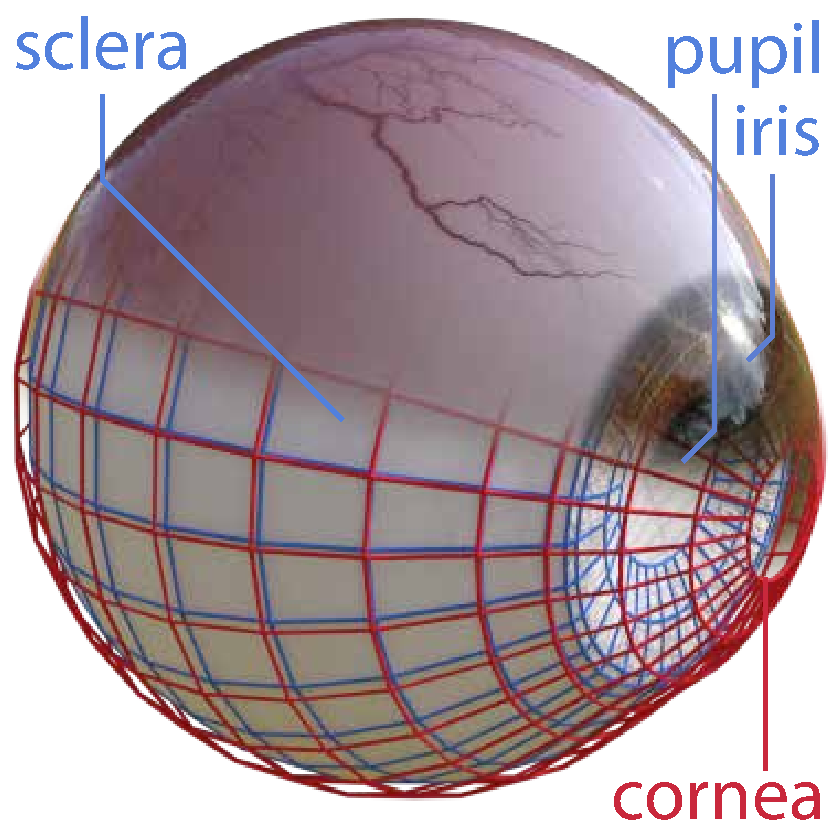
\includegraphics[width=\textwidth]{eye_model}
        \caption{3D eye model}
        \label{fig:3d_eye_model}
    \end{subfigure}%
    \hfill
    \begin{subfigure}[t]{0.65\columnwidth}
        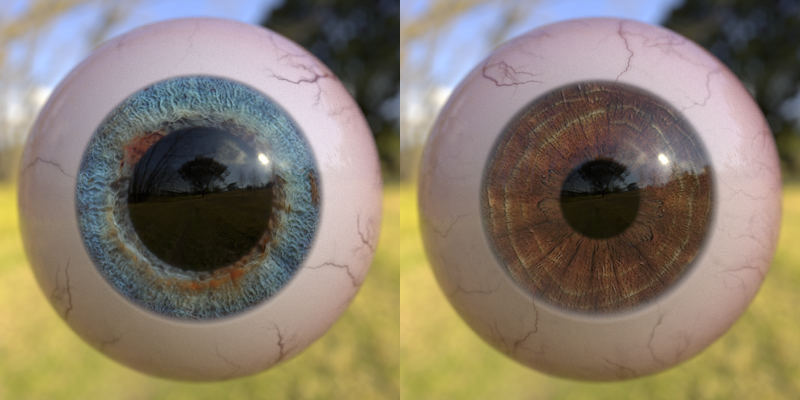
\includegraphics[width=\textwidth]{eye_examples}
        \caption{Pupil dilation and iris color variation}
    \end{subfigure}
    \caption{Our realistic eye model is capable of expressing degrees of variability seen in real life.}
    \label{fig:eye_model}
\end{figure}

Eyeballs are complex organs comprised of multiple layers of tissue, each with different reflectance properties and levels of transparency. Fortunately, as realistic eyes are so important for many areas of CG, there is already a large body of previous work on modelling and rendering eyes \commentE{cite}.

% It is important to accurately model reflections and refractions in the eye as they can lead to specular highlights -- these common eye-region image features are often used by eye-tracking algorithms, or can confound approaches that are not robust.

As shown in \autoref{fig:3d_eye_model}, our eye model consists of two parts.
%
The outer part (red wireframe) approximates the eye's overall shape with two spheres ($r_1\!=\!12\textrm{mm}, r_2\!=\!8\textrm{mm}$ \cite{ruhland2014look}), the latter representing the corneal bulge. To avoid a discontinuous seam between spheres, the meshes were joined and then smoothed. It is transparent, refractive ($n\!=\!1.376$), and partially reflective. The eye's bumpy surface variation is modelled by a displacement map generated with noise functions.
%
The inner part (blue wireframe) is a flattened sphere with Lambertian material. The planar end represents the iris and pupil, and the rest represents the sclera -- the white of the eye.
%
There is a $0.5\textrm{mm}$ gap between the outer and inner parts which accounts for the thickness of the cornea. \commentE{compare with recent Disney work}

Eyes exhibit variations in both shape (pupillary dilation) and texture (iris color and scleral veins). To model shape variation we use \emph{shape keys} -- a CG animation technique where different versions of a mesh are stored, modified, and interpolated between \cite{orvalho2012facial}. We have shape keys representing dilated and constricted pupils, as well as large and small irises to account for a small amount ($10\%$) of variation in iris size.

We vary the appearance of the eye by compositing textures in three separate layers:
\begin{inparaenum}[\itshape i\upshape)]
\item a \emph{sclera} layer representing the tint of the sclera (white, pink, or yellow);
\item an \emph{iris} layer with four photo-textures of different colored irises (amber, blue, brown, grey); and
\item a \emph{veins} layer which varies between blood-shot and clear
\end{inparaenum}. We matched the sclera tint to each separate face model, but uniformably randomly varied iris color. Previous research on iris-synthesis \commentE{cite} would have allowed continually different iris textures, but we decided this added complexity would not make a worthwhile improvement in overall appearance variation, especially when rendered at lower resolutions.

\begin{figure*}
    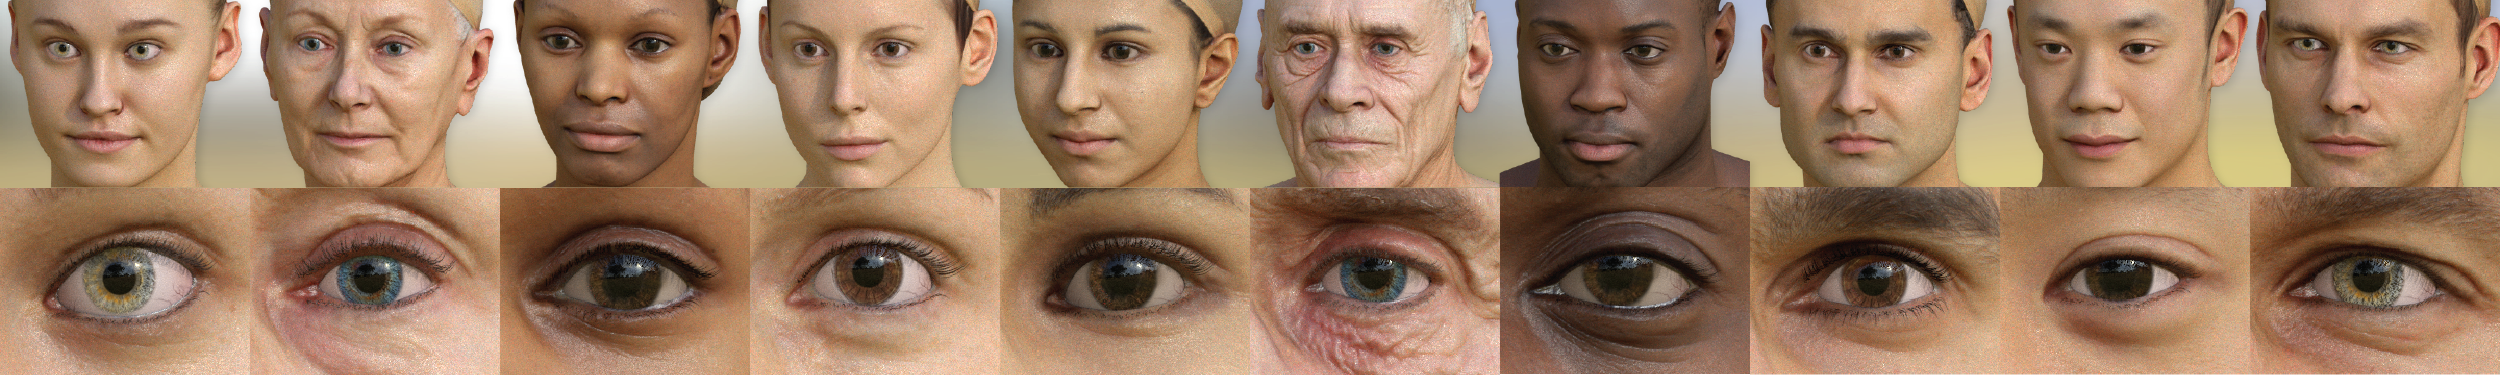
\includegraphics[width=\textwidth]{model_suite}
    \caption{Our suite of female and male head models for rendering.}
    \label{fig:model_suite}
\end{figure*}

\begin{figure*}
    \centering
    \begin{subfigure}[t]{0.195\textwidth}
        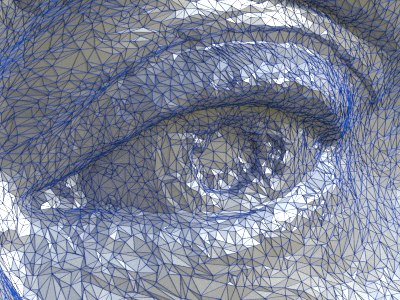
\includegraphics[width=\textwidth]{process_f02_01}
        \caption{Original 3D head scan data: 1.4 million polys}
        \label{fig:process_original_scan}
    \end{subfigure}
    \hfill
    \begin{subfigure}[t]{0.195\textwidth}
        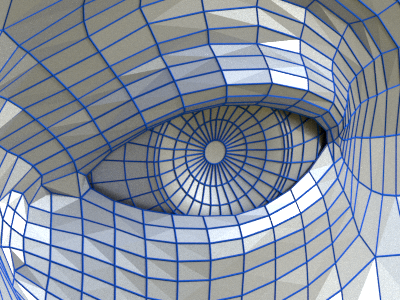
\includegraphics[width=\textwidth]{process_f02_02}
        \caption{Retopologized head model: 9 thousand polys}
        \label{fig:process_retopo}
    \end{subfigure}
    \hfill
    \begin{subfigure}[t]{0.195\textwidth}
        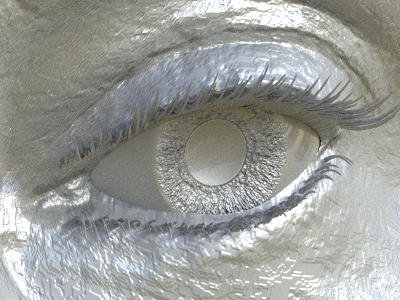
\includegraphics[width=\textwidth]{process_f02_03}
        \caption{Surface detail is stored in displacement maps}
        \label{fig:process_displaced_subdiv}
    \end{subfigure}
    \hfill
    \begin{subfigure}[t]{0.195\textwidth}
        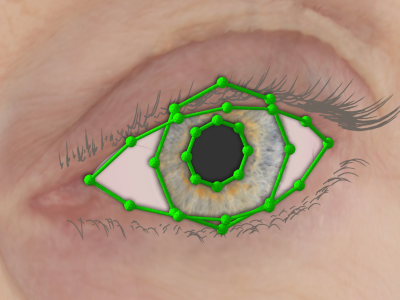
\includegraphics[width=\textwidth]{process_f02_04}
        \caption{3D iris and eyelid landmarks are annotated}
    \end{subfigure}
    \hfill
    \begin{subfigure}[t]{0.195\textwidth}
        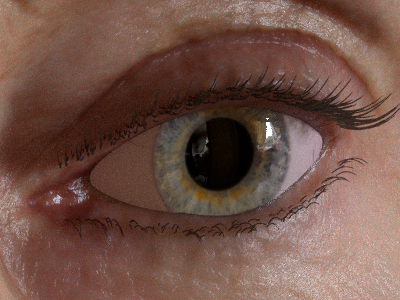
\includegraphics[width=\textwidth]{process_f02_05}
        \caption{The final render}
    \end{subfigure}
    \caption{Model preparation process}
    \label{fig:process}
\end{figure*}

\subsection{Preparing a suite of 3D eye-region models}

Start with 3D head scan data -- a dense mesh.

% Replace eyes
As can be seen in \autoref{fig:process_original_scan}, the cornea has been incorrectly reconstructed in the head scan. This is because transparent surfaces are not directly visible, so cannot be reconstructed in the same way as diffuse surfaces like skin. Recent work uses a hybrid reconstruction method to reconstruct the corneal surface seprately, but requires additional hardware \cite{berard2014highquality} -- this level of detail was deemed unneccesary for our purposes. As we need full control of where the eye looks, we remove the original scanned eyeball from the mesh using boolean operations and place our own eyeball approximation in its place.

% retopo
While the original head scan geometry is suitable for being rendered as a static model, its topology cannot easily represent dynamic changes in eye-region shape. Vertical saccades are always accompanied by eyelid motion \cite{liversedge2011oxford}, so we need to be able to pose the eyelids according to the gaze vector. When preparing a mesh for facial animation, edge loops should flow along and around the natural contours of facial muscles. This leads to a more efficient (lower-resolution) geometric representation of the face, and more realistic animation as mesh deformation mathes that of actual muscles.

We therefore \emph{retopologize} the face geometry into a more optimal form using a commercial semi-automatic system \cite{ZRemesher}. \commentE{Reference some other options, e.g automatic methods in research} As can be seen in \autoref{fig:process_retopo}, edge loops now follow the \emph{Orbicularis Oculi} muscle, allowing for realistic eye-region deformations. This retopologized low-poly mesh now lacks the detail of the original scan (e.g. the crease above the eye), and has visible sharp edges. We therefore use it as the control mesh for a displaced subdivision surface \cite{lee2000displaced}, with displacement map computed from the scanned geometry. As can be seen in \autoref{fig:process_displaced_subdiv}, detail is restored.

Although they are two seperate organs, there is normally no visible gap between eyeball and skin. However, as a consequence of removing the eyeball from the original scan, the retopologized mesh will not necessarily meet the geometry of our eyeball model (\autoref{fig:process_retopo}). To compensate, the face mesh's eyelid vertices are displaced along their normals to their respective closest positions on the eyeball geometry (\autoref{fig:process_displaced_subdiv}). This automatic operation ensures the models are joined, even after changes in pose \cite{Shrinkwrap}.

Eyelashes are short curved hairs that grow from the edges of the eyelids. In CG they are often represented by a curved surface textured with a generic eyelash texture, but we choose to model them using particle effects for a greater degree of control. The hair particles are directed away from the face; the upper eyelashes grow with negative gravity, causing them to point upwards, and the lower eyelids experience a slight gravity to point them downwards.

Add landmarks mesh.

Create face, eyelash, and landmark blend shapes for eyelids looking up and down.

\subsubsection{Eyelid motion}

\begin{figure}
    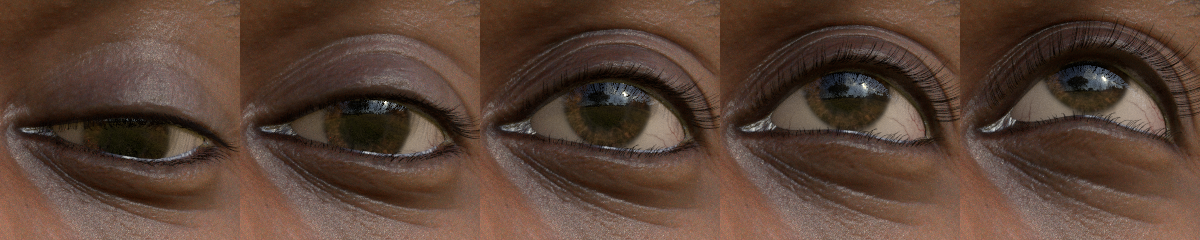
\includegraphics[width=\columnwidth]{eyelid_motion.png}
    \caption{Eyelids.}
\end{figure}



\subsection{Lighting}

\begin{figure}
    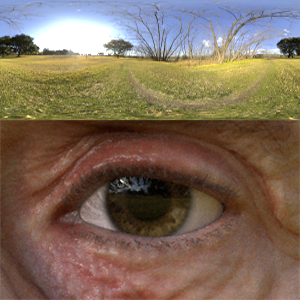
\includegraphics[width=0.24\columnwidth]{fig_env_1} \hfill
    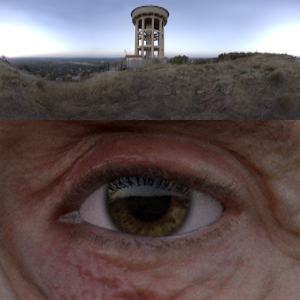
\includegraphics[width=0.24\columnwidth]{fig_env_2} \hfill
    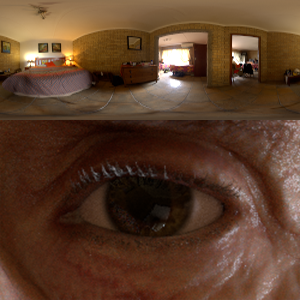
\includegraphics[width=0.24\columnwidth]{fig_env_3} \hfill
    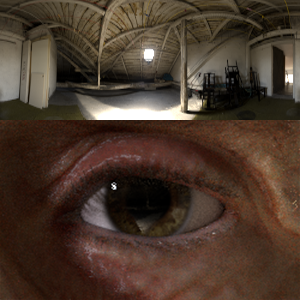
\includegraphics[width=0.24\columnwidth]{fig_env_4}
    \caption{Appearance variation from lighting is modelled with poseable high-dynamic-range environment maps \cite{debevec2002image}.}
    \label{fig:participants}
\end{figure}
